\subsection{Design and static verification of rack and gear}
The verification continued with the parts responsible for actuating the machine, rack that is positioned on both tracks and gear attached on the motors' shaft.
We focused on two important aspects, interference and tooth root bending resistance.

\subsubsection*{Interference condition}
It's fundamental to check if this condition is fulfilled, because otherwise we could have a problem of undercut, when the tip of the rack cutter is moved beyond the base circle of the gear and the result is the weakening of the gear's teeth.

Interference condition is function of the minimum number of teeth of the pinion, in accordance with the following equation:
\begin{equation}
	\centering
	z_{min} = \frac{2}{sin^2\alpha},
\end{equation}
where $\alpha$ is the pressure angle, as we can see in figure \ref{fig:rack}.
\begin{SCfigure}[1][hbt]
	\centering
	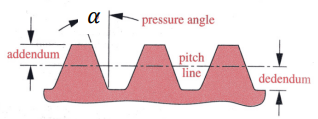
\includegraphics[scale=1]{Images/rack.png}
	\caption{standard rack and pressure angle $\alpha$.}
	\label{fig:rack}
\end{SCfigure}
In our case we designed the profile with a pressure $\alpha = 20^\circ$, thus we have:
\begin{equation*}
	z_{min} = 17,
\end{equation*}

\subsubsection*{Gear design and verification}
	The gear attached to the motor's shaft is designed choosing as number of tooth $z=18$; assuming that the motors actuating the machines can generate a power $P=10W$ at $n = 50rpm$, the associated maximum generated torque is $T=1.9N\cdot m$. Choosing as module $m$ of the gear the value $2mm$, then the nominal diameter of the gear is $d = zm = 36mm$ and the maximum force that can be transmitted by the gear is
	\[ F = \frac T r = 2 \frac T d = 106N\]
	
	\paragraph{Tooth root fatigue resistance}	One of the most important problem in the usage of gears is the teeth fatigue resistance, due to the fact they're subjected to pulsating loads.  
	In our analysis we used the Lewis method that consider the tooth as a cantilever beam and shear and compressive normal stresses are neglected.
	
	According to such theory, the stress state acting on the tooth is
	\[ \sigma = \frac{F}{mb Y_l}\]
	where $b$ is the face width (figure \ref{fig:tooth}) and $Y_l$ is the Lewis factor taking into account for the shape of the tooth; such parameter depends on both the number of teeth $z$ and the pressure angle $\alpha$, and for the given data it evaluates to $Y_l = 0.308$.
	\begin{figure}[bt]
	\begin{subfigure}{.5\textwidth}
		\centering
		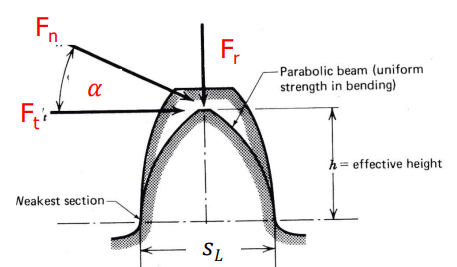
\includegraphics[scale=0.5]{Images/toothgear1.png}
		\caption{}
	\end{subfigure}%
	\begin{subfigure}{.5\textwidth}
		\centering
		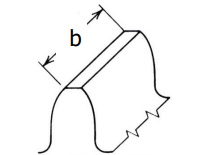
\includegraphics[scale=0.6]{Images/toothgear2.png}
		\caption{}
	\end{subfigure}
	\caption{tooth details: section (a) and face width (b).}
	\label{fig:tooth}
	\end{figure}
	
	Given the ultimate tensile strength $\sigma_{uts} = 40MPa$ of plastic materials used in 3D printing machine and choosing a safety factor $\phi= 2$, reversing the Lewis equation gives us the minimum face width:
	\[ \sigma \leq \frac{\sigma_{uts}}{\phi} \qquad \Rightarrow \qquad b \geq \frac{F \phi}{Y_l m \sigma_{uts}} = 8.61mm \]
	thus a width $b = 10mm$ for the teeth has been chosen.
